%% The first command in your LaTeX source must be the \documentclass command.
\documentclass[acmtog, language=ngerman]{acmart}
\PassOptionsToPackage{english,ngerman}{babel}
%\usepackage[english,ngerman]{babel}
\usepackage[utf8]{inputenc} 

%% \BibTeX command to typeset BibTeX logo in the docs
\AtBeginDocument{%
  \providecommand\BibTeX{{%
    \normalfont B\kern-0.5em{\scshape i\kern-0.25em b}\kern-0.8em\TeX}}}
    
\copyrightyear{2024}
\acmYear{2024}
\citestyle{acmauthoryear}

\usepackage[figurename=Fig.]{caption}
\setcopyright{none}
\makeatletter
\renewcommand{\fnum@figure}{Abb. \thefigure}
\makeatother
\addto\captionsngerman{\renewcommand{\figurename}{Abb.}}
\settopmatter{printacmref=false} % Removes citation information below abstract
\renewcommand\footnotetextcopyrightpermission[1]{} % removes footnote with conference information in first column

%%
%% end of the preamble, start of the body of the document source.
\begin{document}
\selectlanguage{ngerman}

%%
%% The "title" command has an optional parameter,
%% allowing the author to define a "short title" to be used in page headers.
\title{Fähigkeiten und Vorgehen von Low-Code-Ansätzen}

%%
%% The "author" command and its associated commands are used to define
%% the authors and their affiliations.
%% Of note is the shared affiliation of the first two authors, and the
%% "authornote" and "authornotemark" commands
%% used to denote shared contribution to the research.
\author{Teo Förste}
\authornote{Alle Studierenden trugen zu gleichen Teilen zu dieser Arbeit bei.}
\author{Christin Göb}
\authornotemark[1]
\author{Chiara Schepke}
\authornotemark[1]
\affiliation{%
  \institution{\\
Hochschule für Technik, Wirtschaft und Kultur Leipzig}
  \streetaddress{Karl-Liebknecht-Str. 132}
  \city{Leipzig}
  \country{Deutschland}
  \postcode{04277}
}
%%
%% By default, the full list of authors will be used in the page
%% headers. Often, this list is too long, and will overlap
%% other information printed in the page headers. This command allows
%% the author to define a more concise list
%% of authors' names for this purpose.
\renewcommand{\shortauthors}{Förste, Göb, Schepke}

%%
%% The abstract is a short summary of the work to be presented in the
%% article.
\begin{abstract}
  (Abstract-Länge ist typischerweise 15-25 Zeilen lang, in der PDF-Darstellung) 
  
  A clear and well-documented \LaTeX\ document is presented as an
  article formatted for publication by ACM in a conference proceedings
  or journal publication. Based on the ``acmart'' document class, this
  article presents and explains many of the common variations, as well
  as many of the formatting elements an author may use in the
  preparation of the documentation of their work.
\end{abstract}

\maketitle

\section{Einleitung und Motivation}

\begin{figure}[H]
    \centering
    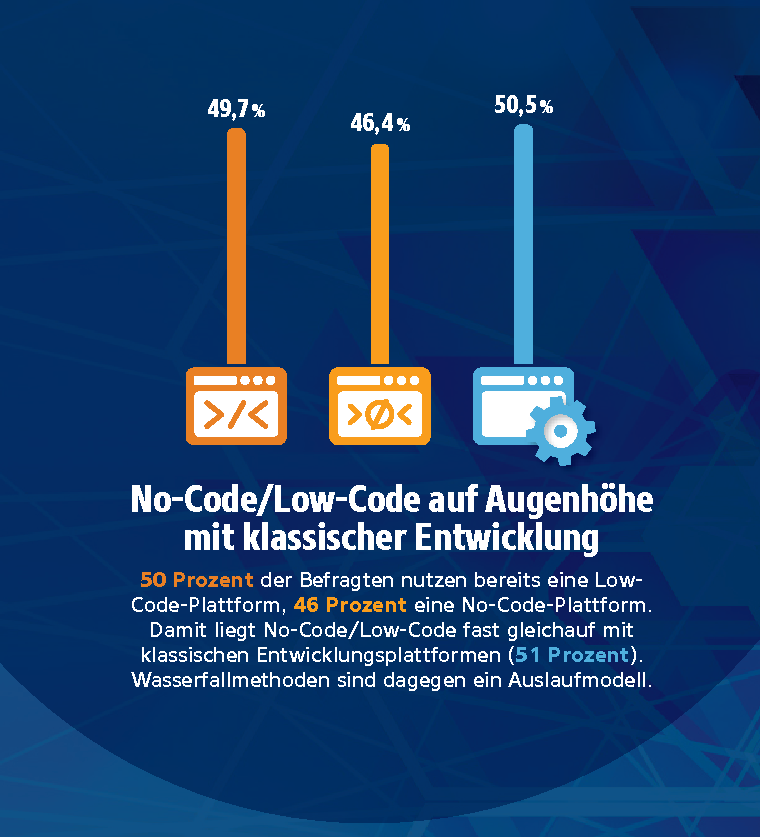
\includegraphics[width=\linewidth]{images/studie-low-code-cropped.pdf}
    \caption{aus \cite{studie_low_code}}
    \label{fig:low_code_no_code}
\end{figure}
%(Beschreibung von Kontext, Problemen, Anforderungen und Zielen)

\subsection{Kontext}
Die mit großen Schritten voranschreitende Digitalisierung auf der einen und der Fachkräftemangel in der IT-Branche auf der anderen Seite begünstigen die Entwicklung und Verbreitung alternativer Methoden zur traditionellen Softwareentwicklung. \cite{flake_fachkraeftemangel_2023} Laut einer aktuellen Studie haben 50 Prozent aller Befragten bereits mit einer Low-Code-Plattform gearbeitet (s. Abb. \ref{fig:low_code_no_code}). Der weltweiten Marktgröße von Low-Code-Plattformen wird eine durchschnittliche jährliche Wachstumsrate von 27,8 Prozent vorhergesagt. Bis 2030 soll sie einen Gesamtwert von 148,5 Milliarden US-Dollar erreichen. \cite{straits_low_code_development_platform_market_2021} 

\subsection{Aufbau und Ziel der Arbeit}
In dieser Arbeit wird zunächst erklärt, was Low-Code Plattformen sind und wie sie sich die Arbeit mit ihnen von der klassischen Softwareentwicklung unterscheidet. Anhand von ausgewählten Szenarien wird aufgezeigt, wie sich die Vor- und Nachteile gegenüber High-Code konkret äußern. Ferner sollen die Grenzen der Arbeit mit Low-Code beleuchtet werden.

%(kurze Zusammenfassung der Struktur der Belegarbeit)

\section{Low-Code}
Dieses Kapitel führt den Begriff Low-Code auf sprachlicher sowie inhaltlicher Ebene ein. Anhand einiger ausgewählter Beispiele aus der Vergangenheit wird aufgezeigt, dass Ansätze aus dem Low-Code schon wesentlich länger Verwendung finden als der Begriff selbst.


\subsection{Terminologie}
Der Begriff setzt sich zusammen aus den Worten low (engl. niedrig) und code. Code meint dabei den Quellcode, während low sich auf die Menge an diesem in einem Softwareprojekt bezieht. "low [amount of] code" bedeutet also, dass nur eine geringe Menge an Quellcode geschrieben werden muss, um eine Software zu entwickeln. Zur Abgrenzung von der klassischen Softwareentwicklung, welche üblicherweise, und insbesondere bei umfangreichen Projekten, eine große Menge an Code benötigt, ist für diese auch der Begriff High-Code geläufig. Eine weitere Variante dieser Namensgebung ist No Code, welche eine extreme Form von Low-Code beschreibt, bei der komplett auf Quellcode verzichtet wird, während Low-Code lediglich versucht, die Menge an Quellcode, welcher von den Entwickelnden per Hand geschrieben werden muss, auf ein Minimum zu reduzieren.

\subsection{Was ist Low-Code?}
In seinem Beitrag "Low-code platform for automating business processes in manufacturing" bezeichnet Robert Wazkowski das Low-Code-Prinzip als eine Weiterentwicklung von Programmiersprachen der vierten Generation (Fourth Generation Language, 4GL) und listet folgende Entwicklungsansätze auf, welche seiner Erkenntnis nach der Low-Code Programmierung zu Grunde liegen:

\begin{itemize}
    \item Modellgetriebene Softwareentwicklung (Model Driven Development, MDD). Dieser stellt das Modell in den Mittelpunkt des Entwicklungsprozesses. Im Gegensatz zur unterstützenden Verwendung von Modellen im Rahmen eines Softwareentwicklungsprozesses, etwa zwecks Veranschaulichung, wird beim MDD der Quellcode semi- oder vollautomatisch aus dem erstellten Modell generiert. Dieser Ansatz findet sich in vielen Implementierungen des Low-Code Prinzips.
    \item Schnelle Anwendungsentwicklung (Rapid Application Development, RAD), siehe Kap. \ref{sec:rad}.
    \item Automatisierte Codegenerierung (Automatic Code Generation) meint die automatisierte Erstellung von Quellcode auf der Grundlage einer höheren Abstraktionsebene. Handelt es sich bei dieser um ein Modell, so kann dieses Verfahren als Ergänzung des modellgetriebenen Entwicklungsansatzes dienen.
    \item Visuelle Programmierung (Visual Programming, VP). Dabei handelt es sich um einen dem Low-Code-Prinzip ähnlichen Softwareentwicklungsansatz. Die Ähnlichkeit besteht im gemeinsamen Ziel, die Menge an manuell zu schreibendem Programmcode zu minimieren sowie dem visuellen Ansatz zum Erreichen dieses Ziels. Während grafische Elemente das Herzstück des visuellen Programmieransatzes darstellen, ist Low-Code hingegen nicht allein auf diese beschränkt.
\end{itemize}

Die Art und Weise, wie die die Menge an von den Entwickelnden selbst zu schreibendem Quellcode bei der Softwarentwicklung konkret minimiert wird, unterscheidet sich im Detail von Plattform zu Plattform. Üblich ist die Verwendung einer grafischen Benutzeroberfläche im Gegensatz zum Quellcodeeditor bei der High-Code Entwicklung.

Das Forschungsteam um Davide Di Ruscio hat in einem Expert Voice Paper für die IFAC untersucht, ob es sich bei Low-Code nicht einfach nur um eine neue, alternative Bezeichnung für den bereits bekannten modellgetriebenen Entwicklungsansatz handelt. Dabei kamen die Forschenden zu dem Ergebnis, dass sich die beiden Vorgehensweisen zwar in vielen Belangen ähneln, im Grunde aber dennoch zwei unterschiedliche Programmierkonzepte darstellen. \cite{low_code_vs_mdd}

\subsection{Low-Code-Ansätze in der Vergangenheit}
Erstmals eingeführt im Jahr 2011, beschreibt der Begriff Low-Code ein modernes sowie, basierend auf den Ergebnissen der Studie \cite{studie_low_code}, durchaus zukunftsfähiges Entwiklungskonzept. Nichtsdestotrotz offenbart ein Blick in die Geschichte, dass einige Ansätze aus dem Low-Code bereits seit Jahrzehnten zur Anwendung kommen und Entwickelnden ihre Arbeit erleichtern.

Bei folgenden Beispielen handelt es sich um Softwareentwicklungstools aus den 80er- und 90er-Jahren, welche eines oder mehrere Merkmale aufweisen, die nach heutiger Definition dem Low-Code-Entwicklungsansatz inhärent sind. Es handelt sich ausdrücklich nicht um Low-Code-Plattformen.

\subsection{Eine neue Zielgruppe}
Die modellgetriebene Natur des Low-Code Entwicklungsansatzes und der Verzicht auf die Notwendigkeit von handgeschriebenem Code ermöglichen es auch informationstechnischen Laien ohne Programmierkenntnisse, Software zu entwickeln. Für diese neue Form der Softwareentwickelnden hat sich der Begriff "Citizen Developer" etabliert. In ihrer Studie "The Rise of the Citizen Developer" beschreiben Marten Oltrogge et al. Citizen Developer als "developers with little or no software engineering background", also Entwickelnde mit wenig oder gar keiner Erfahrung im Software Engineering. \cite{oltrogge_2018}

Die Anbieter von Low-Code Entwicklungsumgebungen unterstützen die Erschließung dieser neuen Zielgruppe durch die Bereitstellung weiterer Werkzeuge und Dienstleistungen. \cite{low_code_vs_mdd}

Die Betreiber der Low-Code Plattform FlutterFlow werben auf ihrer Website unter anderem mit folgenden Funktionen: \cite{flutterflow_features}

\begin{itemize}
    \item Versionskontrolle durch Branching
    \item Erstellen von Tests für die einzelnen Komponenten
    \item Bildschirmaufnahmen (z. B. zwecks Marketing)
    \item Cloud-Funktionalitäten mit Firebase
\end{itemize}

Auch Arbeitsschritte, die über den eigentlichen Entwicklungsprozess hinausgehen, wie etwa die Veröffentlichung des fertigen Produkts auf verschiedenen Plattformen, werden als Dienstleistung angeboten.\cite{flutterflow_deployment} Mit einem solchen Rundumpaket können sich die Citizen Developer voll und ganz auf den Aufbau, die Struktur, das Design und die Funktionalität ihrer Software konzentrieren. Welche Nachteile dieses Entwicklungskonzept gegebenenfalls mit sich bringen kann, wird im weiteren Verlauf dieser Arbeit thematisiert.

\section{Begrifflichkeiten im Zusammenhang mit Low-Code-Entwicklung}



\subsection{Rapid Application Development} \label{sec:rad}

Rapid Application Development, nachfolgend RAD abgekürzt umfasst eine Methode der Softwareentwicklung, die speziell darauf abzielt, Anwendungen schnell und effizient zu erstellen. Der Fokus dabei liegt auf der schnellen Bereitstellung funktionsfähiger Software, wobei iterative Prozesse, die Beteiligung von Endbenutzer:innen und die Wiederverwendung von Softwarekomponenten im Vordergrund stehen.
Die Merkmale von RAD lassen sich wie folgt kategorisieren. Schnelle Iterationen, benutzerzentrierter Ansatz, Wiederverwendung von Komponenten, Protoyping, flexible Anpassung an Änderungen und visuelle Entwicklung. \cite{rapid_protoyping}

RAD und das MVP ergänzen sich in den meisten Punkten und können deshalb gut gemeinsam eingesetzt werden.



\section{Vorgehensweisen in Software Projekten}

Nachdem die grundlegenden Konzepte von Low-Code im vorigen Abschnitt behandelt wurden, werden im folgenden Abschnitt verschiedene Szenarien beschrieben, an denen dargestellt wird, wie ein Software Unternehmen Low-Code einsetzen kann. Hierbei werden gängige Methodiken der Softwareentwicklung benannt und die Vorteile beziehungsweise Nachteile die sich durch die Verwendung von Low-Code-Ansätzen aufgezeigt.

\subsection{Low-Code in großen Software Unternehmen }

Gängige Problematiken die bei der Entwicklung von Software, unabhängig von der Größe des Teams, auftreten können sind: 
\begin{itemize}
\item Warten von Bestands-Code

Während der Laufzeit müssen Ressourcen aufgebracht werden, um Software lauffähig zu halten. Je länger die Laufzeit, desto höher das Risiko, dass der Sourcecode veraltet und eventuelle Sicherheitslücken auftreten. 

Das Erweitern von Bestands-Code durch neue Funktionalitäten birgt ebenfalls verschiedene Hürden. Eventuell existiert keine ausreichende Dokumentation, durch mangelnden Überblick seitens der Entwickler können Änderungen neue Probleme erzeugen, statt positive Effekte zu erzielen.

\item Dependency Management

Es muss beachtet werden, dass Dependencies regelmäßig geupdatet werden müssen, um gewährleisten zu können, dass keine Kompatibilitätsprobleme und  Sicherheitslücken auftreten können.

\item Kompatibilitätsprobleme

Wird nicht auf Kompatibilität geachtet, kann es schon während der Entwicklung eines Projektes zu Problemen mit unterschiedlichen Plattformen, Browsern und Komponenten von Drittanbietern kommen. 

\item Managen von Test Automation und Test Environments

Tests sollten in jeder Stufe der Entwicklung genutzt werden, um die Qualität des Produktes und des Codes zu prüfen.

\item Scalability

Software muss Veränderungen in der Menge der User-Anfragen und Data-Loads standhalten können.

\item Security Concerns

Mögliche Sicherheitslücken müssen erkannt und geschlossen werden. 

\item Gesetzliche Regulationen

Neue Gesetzliche Vorschriften, wie die DSGVO, müssen in der Software-Entwicklung berücksichtigt und umgesetzt werden.

\item Fachkräftemangel

Der Mangel an ausgebildetem Fachpersonal muss in der Planung von Software-Projekten berücksichtigt werden.

\item Wissensweitergabe \& Onboarding

Wenn neue Personen Teil eines Teams werden und andere Personen in ihrer Funktion 

\item Kommunikation

Je größer ein Projekt, ein Entwicklungsteam oder ein Unternehmen ist, desto mehr Personen müssen miteinander kommunizieren. Hierbei können mehrere Probleme auftreten.
Wenn ein Unternehmen viele Projekte umsetzt, liegen diesen oft unterschiedliche Anforderungen zugrunde. Wenn nun neue Standards eingeführt werden sollen, können diese in einem der Projekte sehr leicht, im nächsten nur sehr schwer umsetzbar sein. 
Teilweise müssen Unternehmensweite Veränderungen von Coding-Standards koordiniert werden. Teams können untereinander Konkurrieren und Anforderungen völlig unterschiedlich interpretieren und umsetzen. Manche Projekte arbeiten eventuell gegeneinander. 
\end{itemize}

\subsection{Aktuelle Nutzung von Low-Code}
Eine Studie aus München aus 2023 wurde mit 386 Teilnehmenden durchgeführt. \cite{studie_low_code}  Dabei sind diese jeweils aus verschiedenen Branchen 
an der insgesamt 386 interviews mit personen aus verschiedenen branchen durchgeführt wurden. von diesen sagten …

386 Teilnehmende insgesamt. 

Von 295 Befragten geben 68,8\% an, dass die Coronapandemie, der Ukraine-Krieg und ähnlich gewichtige Ereignisse und Entwicklungen in den letzten Jahren einfluss auf den Einsatz von low-/und no-code Lösungen haben.


\subsection{Minimum Viable Product}
Ein zentraler Aspekt der agilen Software-Entwicklungs-Methodik ist das Minimum Viable Product, nachfolgend MVP abgekürzt. Es ist eine bestimmte Art und Weise, wie ein Softwareentwicklungsprojekt organisiert werden kann.
Das Grundprinzip des MVP ist es, früher Zufriedenheit beim Kunden zu schaffen und kontinuierliches Optimieren umzusetzen. In die deutsche Sprache übersetzt, bedeutet MVP, dass es darum geht, die minimale mögliche Umsetzung eines Softwareprojekts zu finden.

\begin{figure}[h]
    \centering
    
\includegraphics[width=1\linewidth]{images/mvp_grafik.jpg}
    \caption{Agiles Vorgehen: MVP-Gedanke \cite{mvp_definition}}
    \label{fig:enter-label}
\end{figure}
Die Abbildung Nummer 1 von Marty True \cite{mvp_definition} soll zeigen, dass es insgesamt bei der agilen Methodik darum geht, ständig an der Grundidee weiterzuarbeiten. Das geplante bzw. entwickelte Produkt soll immer weiter optimiert werden.
Dabei ist wichtig, dass das MVP immer ein Produkt ist, welches von Grund auf funktioniert. Es existiert eine sehr hohe Wahrscheinlichkeit, dass dabei einige Funktionen des Produkts reduziert werden müssen, um dies zu gewährleisten.
Im Fokus dieser Methodik steht also, sich erst einmal ausschließlich auf das zu fokussieren, was wirklich benötigt wird. Das minimale Produkt zu finden, was die grundlegenden Bedürfnisse stillt, ist das Ziel dieser Methodik.
Bei dieser Herangehensweise geht es nicht darum, den Kunden bzw. die Kundin  glücklich zu machen, sondern dass man im Prozess lernt, welche Anforderungen an das Produkt gestellt werden.

Das Prinzip des MVP beschränkt sich nicht auf die erste Iteration und den ersten Prototypen. Es kann immer weiter optimiert werden und würde sich dann bspw. MVP-\textit{X} und dann MVP-\textit{X+1} nennen. Es muss immer sichergestellt werden, dass das jeweilige MVP einsatzfähig ist.

\subsection{Low-Code MVPs}

Firma A möchte, dass für ihre neue Produktlinie ein Online-Shop entwickelt wird. Da die Produkte schon produziert werden, möchten die Stakeholder, dass der Shop schnellstmöglich produktiv genutzt werden kann.

Das Entwicklungsteam hat bisher ausschließlich native Apps mit Hilfe des Frameworks Flutter entwickelt. Der Webshop verkörpert die erste Web App, die das Team entwickelt. Um Zeit zu sparen, wird die Entscheidung getroffen, FlutterFlow zu verwenden. In wenigen Arbeitsstunden soll ein MVP (Minimum Viable Product) entwickelt werden, damit so schnell wie möglich ein funktionaler Webshop angeboten werden kann.

In High-Code-Projekten ist es wichtig sich zu Beginn eines neuen Projektes, insbesondere wenn neue Technologien eingesetzt werden, mehrere Fragen zu beantworten: 

\begin{itemize}
    \item Wie ist das neue Projekt in die bereits bestehende Systemlandschaft integrierbar? 
    \item Welche Sicherheitslücken müssen beachtet und geschlossen werden?
    \item Wie lässt sich Maintainability garantieren? 
    \item Wie kann Source zu einem späteren Zeitpunkt erweitert werden? 
    \item Wie setzt man die Anbindung von Frontend an Backend um? 
    \item Welche Schnittstellen müssen erweitert/angepasst/neu entwickelt werden? 
\end{itemize}

Low-Code-Anbieter scheinen Lösungen für diese Themen zu bieten, jedoch kann dies zu einer starken Abhängigkeit führen. Unternehmen sollten abschätzen, wie aufwändig eine Migration in ein anderes System im Falle einer Auflösung des Low-Code-Anbieters ist. 

Nachdem Firma A die geforderten MVPs umgesetzt hat, ergibt sich für das Entwicklungsteam die Möglichkeit, die Entwicklung auf unterschiedliche Arten fortzuführen. Für den Fall, dass Funktionalitäten durch Low-Code nicht wie gewünscht umsetzbar sind, bieten Low-Code-Anbieter die Möglichkeit einzelne Funktionalitäten mit Hilfe von High-Code-Fragmenten zu entwickeln. Falls dies nicht ausreicht, bietet FlutterFlow einen Export des von der Plattform generierten Flutter-Sourcecodes an. Erfahrene Flutter-Entwickler:innen können diesen Code wie herkömmlichen High-Code behandeln.

Im Falle des beschriebenen Szenarios ist eine Abhängigkeit nur über die Zeit, in der die ersten Versionen und Erweiterungen des MVPs entwickelt werden. Da die Nutzung des Low-Code-Anbieters also auf einen beschränkten Zeitraum innerhalb der Projektlaufzeit genutzt wird, sollten keine Probleme durch eine Abhängigkeit vom Low-Code-Anbieter auftreten.

\subsection{Low-Code-Prototypen}

Das UX-Team von Firma A möchte für eine neue App Prototypen entwickeln, um damit User-Tests durchzuführen. In vergangenen Projekten wurden im Team mit gängigen UI \& UX Tools Prototypen entwickelt, welche für User-Tests genutzt wurden. Nach deren Abnahme wurden diese an die Entwicklungsabteilung gegeben, um anschließend mit High-Code umgesetzt zu werden. Für die neuen Prototypen entscheidet sich das Team jedoch dafür, die Prototypen direkt vom UX-Team als Low-Code MVPs umzusetzen, um High-Code-Entwickler-Kapazitäten zu sparen. 

Des Weiteren bietet die Verwendung von Low-Code-Technologien die Möglichkeit, Prototypen schnell mit Funktionalitäten auszustatten oder direkt MVPs von UX/UI-Designern als Citizen-Developers umsetzen zu lassen, auch wenn diese keine bisherigen Erfahrungen mit Programmieren haben. 

With low-code/no-code tools, it’s more likely that the solution built will work for the people using it. 
ow code tools aren’t a substitute for thinking carefully about the problem.

Related to this idea of eliminating translation issues, low-code tools make prototyping exceptionally easy.
(https://medium.com/u-s-digital-response/strengths-and-weaknesses-of-low-code-no-code-tools-e3e3732b573e)


\subsection{Low-Code und SCRUM-Sprints}

Firma A geht in ihrem High-Code Entwicklungsprozess nach der agilen SCRUM Methode vor. Sogenannte Sprints werden für eine jeweiligen Umfang von zwei Wochen geplant. Innerhalb dieser soll eine festgelegte Auswahl von Features, oder Teile von diesen, umgesetzt werden.

Um Low-Code in ihren Entwicklungsprozess zu integrieren, entscheidet das Entwicklungsteam, während der Entwicklung von MVPs in Low-Code-Umgebungen, den Load der Sprints anzuheben, da sich die gewünschten Features in Low-Code deutlich schneller umsetzen lassen sollten als wie gewohnt in High-Code. Es muss davon ausgegangen werden, dass zu einem fortgeschrittenen Zeitpunkt des Projekts dieser wieder Load abgesenkt werden muss, um das Low-Code-Projekt mit Custom Code zu erweitern.

\subsection{Low-Code und Brand-Design-Änderungen}

Eine Firmengruppe, für die Firma A mehrere Low-Code-Projekte umgesetzt hat, verändert nach mehreren Jahren ihr Brand-Design. Alle Designs dieser Projekte sollen gleichzeitig angepasst werden. Da der gewählte Low-Code-Anbieter eine zentrale Verwaltung von sogenannten Design Themes anbietet, lassen sich durch wenige Schritte alle Designs simultan anpassen.

Vergleichsweise muss bei High-Code Projekten von Anfang an berücksichtigt werden, dass UI und UX Design nach einer längeren Laufzeit des Projektes angepasst oder vollständig verändert werden müssen. Hierfür muss entschieden werden, welches Framework genutzt werden soll, um das Anfangs gewünschte Design umzusetzen und in welchem Rahmen es anpassbar sein soll. Die hierfür getroffenen Rahmenbedingungen müssen von allen Personen, die an dem Sourcecode mitwirken, eingehalten werden, damit spätere Änderungen schnell vorgenommen werden können. 

\begin{figure}[h]
    \centering
    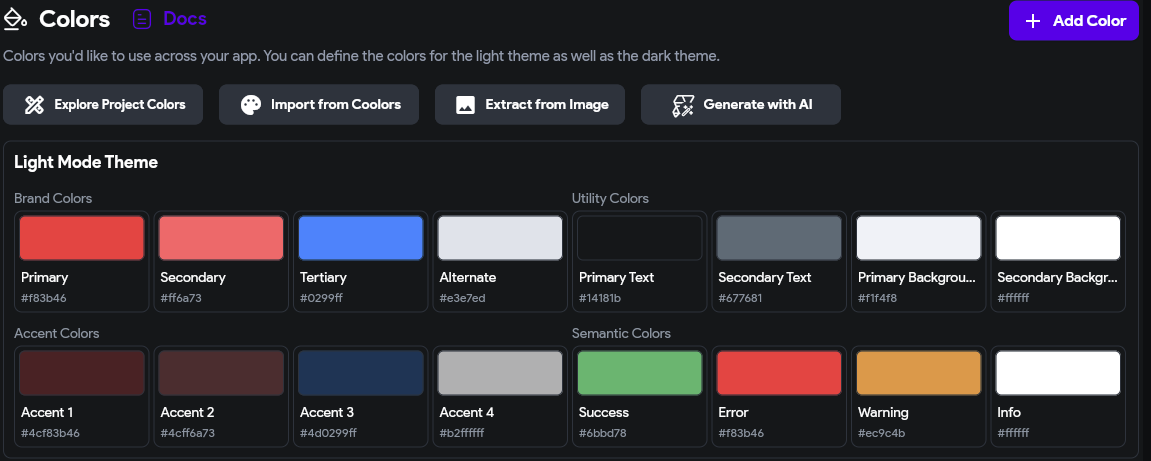
\includegraphics[width=1\linewidth]{Screenshot 2024-01-27 at 15.38.16.png}
    \caption{Ausschnitt der Theme Settings von FlutterFlow}
    \label{fig:enter-label}
\end{figure}

FlutterFlow bietet verschiedene Theme Settings. Darunter fallen die Farbeinstellung. Abbildung 2 zeigt einen Ausschnitt dieser. Das Light Mode Theme beschreibt die als Standard verwendete Farbauswahl der App. Es gibt zu dem ein alternatives Dark Mode Theme, welches von Apps verwendet wird, wenn der User entsprechende Einstellungen im Native-System oder in der App vorgenommen hat. Der Dark Mode bietet meist eine alternative Darstellung von User Interfaces, die deutlich dunkler als die Standardversion ist oder einen dunklen Hintergrund mit heller Schrift nutzt. 

Die Themes bestehen jeweils aus einer Vorauswahl von Farben, die jeweils nach ihrem Nutzungszweck benannt sind. Der Primary Farbton zum Beispiel wird im Verhältnis zu den darauf folgenden Secondary- und Tertiary-Ton am meisten in den Oberflächen der App vorkommen. Sematic Colors werden in spezifischen Fällen angewandt, in denen Zustände mit Farben assoziiert werden, wie zum Beispiel Rot im Fall eines Fehlers verwendet wird. 

Welche Farben genau verwendet werden sollen, lässt sich vom User mit Hilfe eines Farbauswahl-Tools anpassen, es können auch Hashcodes oder RGB-Werte angegeben werden, die die gewünschten Farben beschreiben. 

Die gewählten Farben sind auf der Theme Settings Seite deutlich erkennbar, hierdurch lässt sich abschätzen, ob diese miteinander Harmonieren oder nicht zusammen passen.

\begin{verbatim}
class LightModeTheme extends FlutterFlowTheme {
  @Deprecated('Use primary instead')
  Color get primaryColor => primary;
  @Deprecated('Use secondary instead')
  Color get secondaryColor => secondary;
  @Deprecated('Use tertiary instead')
  Color get tertiaryColor => tertiary;

  late Color primary = const Color(0xFF4B39EF);
  late Color secondary = const Color(0xFF39D2C0);
  late Color tertiary = const Color(0xFFEE8B60);
  late Color alternate = const Color(0xFFE0E3E7);
  late Color primaryText = const Color(0xFF14181B);
  late Color secondaryText = const Color(0xFF57636C);
  late Color primaryBackground = const Color(0xFFF1F4F8);
  late Color secondaryBackground = const Color(0xFFFFFFFF);
  late Color accent1 = const Color(0x4C4B39EF);
  late Color accent2 = const Color(0x4D39D2C0);
  late Color accent3 = const Color(0x4DEE8B60);
  late Color accent4 = const Color(0xCCFFFFFF);
  late Color success = const Color(0xFF249689);
  late Color warning = const Color(0xFFF9CF58);
  late Color error = const Color(0xFFFF5963);
  late Color info = const Color(0xFFFFFFFF);
}
\end{verbatim}


Der Vorangehende Sourcecode-Ausschnitt stellt den zugehörigen, von FlutterFlow generierten Dart-Code dar. Für das LightTheme wird eine Klasse definiert, die Color Datenfelder beinhaltet. Jedes dieser Felder steht für eine andere Farbe des Themes, zum Beispiel die Primary Farbe. Die Farben selbst sind als Hexadezimalzahlen definiert. Für Personen, die den Sourcecode lesen, ist es schwer nachzuvollziehen, um welche Farben es sich bei den Werten genau handelt.


\subsection{Low-Code und App-Deployment}


\section{FlutterFlow - persönliche Einschätzung}

Nachdem einige Zeit mit der Plattform FlutterFlow an einem MVP für einen E-Shop gearbeitet wurde, sind die ein oder anderen Auffälligkeiten deutlich geworden. Diese Auffälligkeiten sind zum großen Teil auch persönliche Einschätzungen und sollen in den nachfolgenden Unterkapiteln aufgezeigt werden.
Außerdem sind alle in diesem Kapitel verwendeten Abbildungen Screenshots der FlutterFlow-Umgebung. Sie stammen aus der Zeit von Dezember 2023 bis Februar 2024.

\subsection{FlutterFlow}
FlutterFlow wurde im Zuge der Arbeit für das Testen einer Low-Code Plattform verwendet und soll an dieser Stelle nur kurz erläutert werden.

FlutterFlow ist eine webbasierte, visuelle Entwicklungsplattform, die auf dem Flutter-Framework von Google basiert. FlutterFlow wurde von zwei ehemaligen Google-Ingenieuren gegründet. Es soll Designer:innen, Entwickler:innen und Unternehmen ganz allgemein das Erstellen mobiler Apps erleichtern.

Die Plattform bietet die Möglichkeit, Entwickler:innen, auch ohne tiefgreifende Programmierkenntnisse, plattformübergreifende mobile Anwendungen zu erstellen.
Flutterflow integriert Backend-Funktionen. Das bedeutet, dass Entwickler:innen grundlegende Server- und Datenbankenfunktionalitäten ohne separate Backend-Entwicklung implementieren können. \cite{flutterflow_features}

\subsection{Visuelle Programmierung}
Die Plattform ist für den Einstieg in die Thematik (Web-)App-Programmierung sehr gut geeignet. Auch ohne Vorkenntnisse mit der Programmiersprache Dart, die FlutterFlow bzw. Flutter verwendet, kann eine vollständig funktionsfähige Applikation entwickelt werden, ohne auch nur eine Zeile Code je gesehen zu haben.

\subsection{Erste Erfolge}
Beim Arbeiten mit FlutterFlow wird sofort deutlich, dass man sehr schnell Ergebnisse sehen kann. Die Entwicklungsumgebung hilft dem Entwickler bzw. der Entwicklerin die Rahmenbedingungen für das Projekt so schnell wie möglich abzunehmen, sodass sich darum nur ganz kurz gekümmert werden muss.
Dabei kann man ganz einfach entscheiden, ob man die (Web-)App vollständig nach seinen eigenen Wünschen umsetzen möchte, oder Templates verwenden möchte.
\begin{figure}[h]
    \centering
    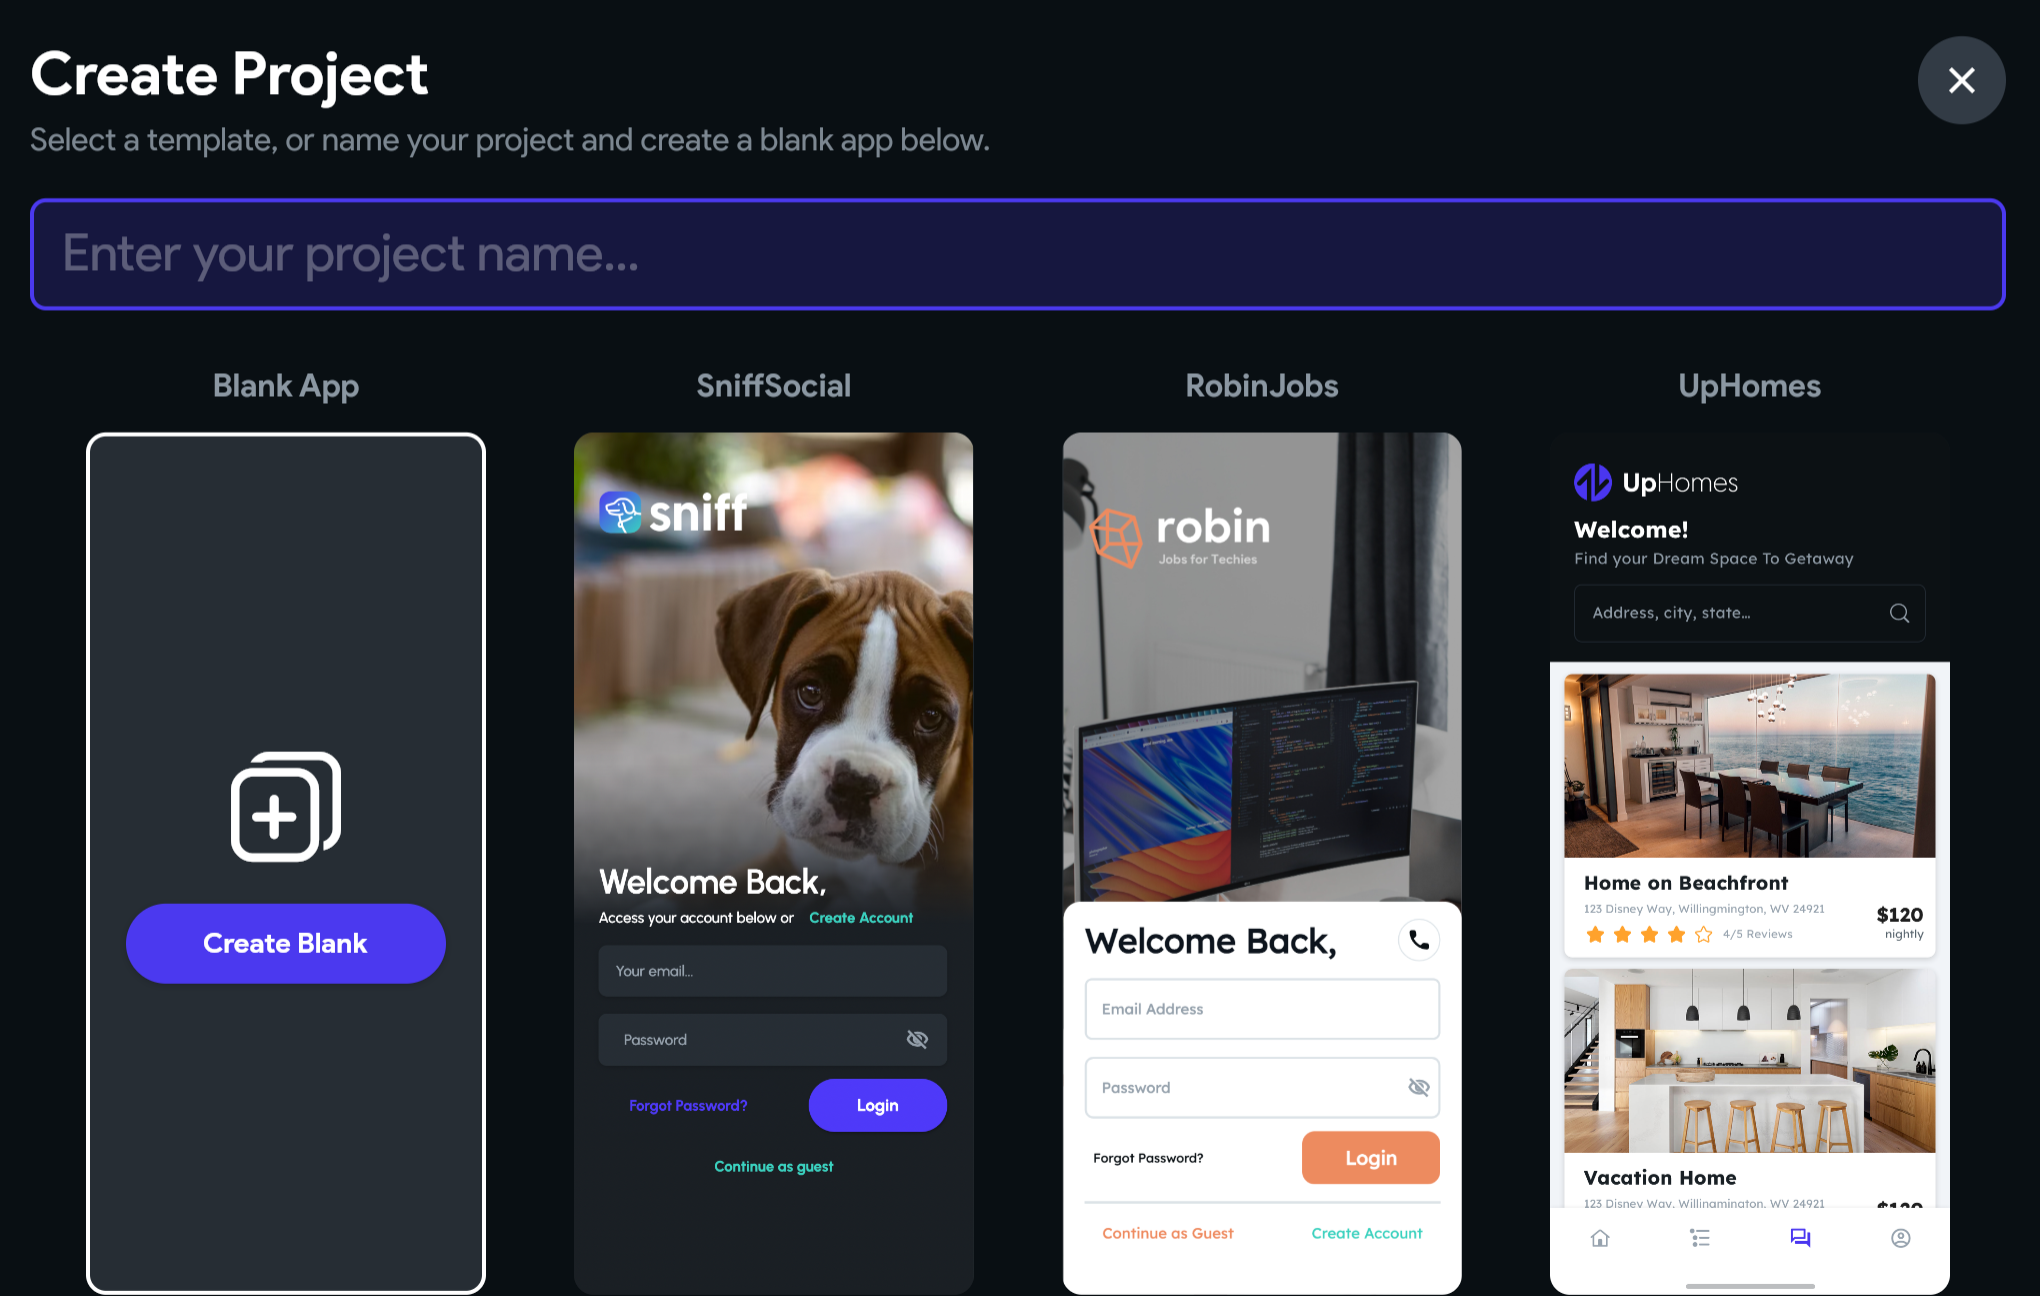
\includegraphics[width=1\linewidth]{images/FF_projekt_erstellen.png}
    \caption{Projekt erstellen FlutterFlow}
    \label{fig:enter-label}
\end{figure}
Hat man sich dann entschieden und die ersten Pages sind erstellt, kann man relativ zügig Elemente aus der "Widget Palette" auf die gewünschte Seite an die gewünschte Stelle ziehen.
\begin{figure}[h]
    \centering
    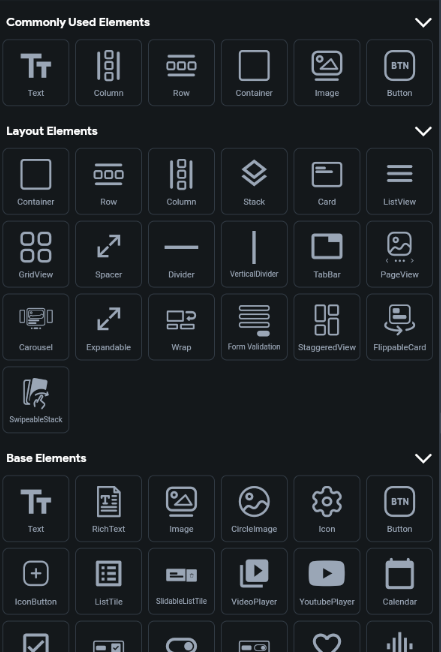
\includegraphics[width=1\linewidth]{images/FF_widget_palette.png}
    \caption{Widget Palette}
    \label{fig:enter-label}
\end{figure}

\subsection{Hinweise}
Schnell wird deutlich, wenn man Fehler macht und bspw. ein Problem erzeugt, was die (Web-)App zum Absturz bringen würde, gibt die Plattform Hinweise diesbezüglich und verhindert den Vorgang. Auch gibt die Plattform Hinweise darüber, wie die User Experience optimiert werden könnte durch bspw. Vorgaben zum Format etc.
\begin{figure}[h]
    \centering
    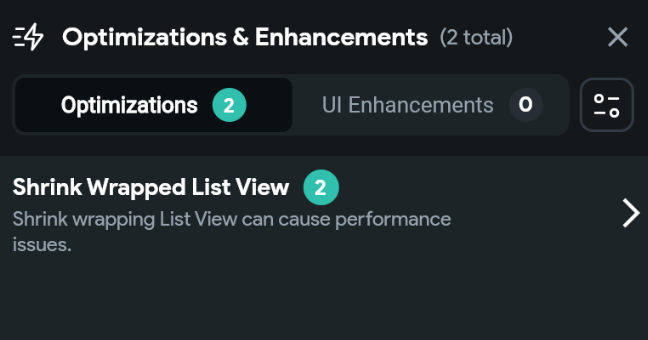
\includegraphics[width=1\linewidth]{images/FF_optimization.png}
    \caption{Optimization \& Enhancement}
    \label{fig:enter-label}
\end{figure}

\subsection{Eingeschränkte eigene Anpassungsmöglichkeiten}
Bei der Arbeit an dem MVP für diesen E-Shop sind keine Einschränkungen aufgetaucht, weil es sich hierbei nur um eine sehr heruntergebrochene Version der Applikation handelt. Es sei jedoch nicht aus den Augen zu verlieren, dass No-Code bzw. Low-Code Plattform bestimmte Vorgaben, Vorlagen und Widgets haben, die zwar abgeändert werden können, wenn es aber darauf ankommt, eine hochgradig spezifische und angepasste Funktion oder Design zu implementieren, es zu Problemen kommen kann. Das liegt daran, dass nur begrenzt Kontrolle über den Code besteht, da dieser zum großen Teil automatisch generiert wird.

An einer Stelle sollte eine Anpassung gemacht werden, die ein wenig Code-Verständnis mit sich bringen sollte.
Im Warenkorb sollte eine Funktion geschrieben werden, die die Summe des Gesamtbetrags abändert, wenn man das bestimmte Produkt aus dem Warenkorb entfernt. Dafür wurde auf die Variable "price" aus dem Document "product" und auf den App State "cartSum". An dieser Stelle musste eine "Code Expression" hinzugefügt werden, da es bei FlutterFlow bei der Increment/Decrement Click-Funktion keine Möglichkeit gibt, eine Variable von einer anderen Variable abzuziehen. Das ganze sieht man dann in Abbildung XX.
\begin{figure}[h]
    \centering
    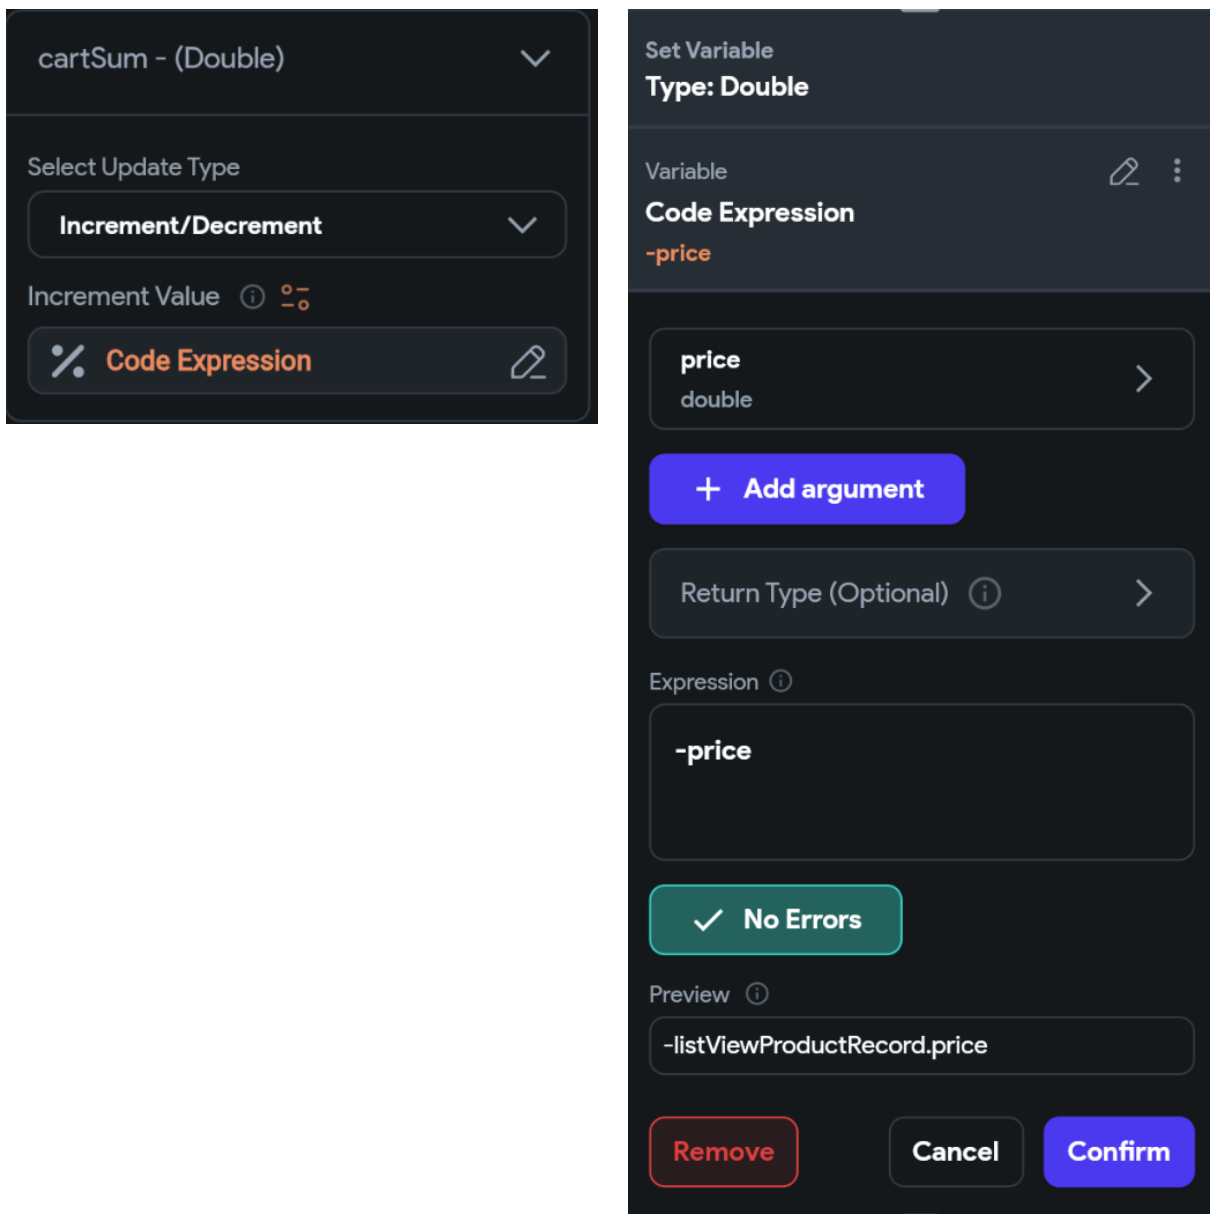
\includegraphics[width=1\linewidth]{images/FF_decrement.png}
    \caption{Warenkorb Decrement Funktion}
    \label{fig:enter-label}
\end{figure}
\subsection{Community und Support}
Beim Arbeiten mit FlutterFlow und beim Fehler beheben fällt schnell auf, dass relativ schnell triviale Probleme gelöst werden können durch Forums-Diskussionen der Community und Informationen von Flutter selbst durch eigene Dokumentationen. Hierbei wird vor allem auf die "FlutterFlow Introduction" verwiesen, die eine Schritt-für-Schritt-Anleitung bietet, um ein erstes eigenes Projekt umzusetzen.

Außerdem bietet der FlutterFlow-Kanal auf YouTube eine hohe Anzahl an Tutorials. Dort werden unter anderem auch ganze Live-Streams zur Verfügung gestellt um bei größeren Projekten mitzuarbeiten. Ein Beispiel: \cite{flutterflow_youtube}


\section{Zusammenfassung und Ausblick}

(Überblick über die gesamte Arbeit, Rückführung auf Aussagen aus Kapitel 1 durchführen, offene Punkte als neue Forschungsfragen definieren)

Zusammenfassend ist zu sagen

%% The next two lines define the bibliography style to be used, and
%% the bibliography file.
\bibliographystyle{ACM-Reference-Format}
\bibliography{quellen}


%% If your work has an appendix, this is the place to put it.
\appendix

\section{Anhang}

\subsection{Übungsaufgaben}
\subsubsection{Aufgabe 1}
Anwenden von FlutterFlow. Öffnen Sie folgende URL um das genannte Projekt zu öffnen, Sie finden den dazugehörigen generierten Sourcecode in folgendem Git Repository: 
Alternativ können Sie ein eigenständiges FlutterFlow Projekt anlegen, oder eines der vorhandenen Beispielprojekte verwenden. Verknüpfen Sie das Projekt mit einem Github Account, eine Anleitung hierzu finden Sie im Developer Menu Ihres FlutterFlow Projektes. 
Suchen Sie nun im Sourcecode nach verschiedenen Komponenten des Projektes.

\subsubsection{Aufgabe 2}
Ändern Sie in diesem Projekt den App-Namen und machen Sie generelle Design-Änderung.

\subsubsection{Aufgabe 3}
Entwickeln Sie eine minimalistische To-Do-Liste mit der Hilfe von FutterFlow. Die App sollte grundlegende Funktionen zum Hinzufüge, Anzeigen und Löschen von Aufgaben bieten.
Gehen Sie dabei auf folgenden Aspekte ein:
\begin{enumerate}
    \item Benutzeroberfläche
    \item Funktionalität
    \item Datenbankintegration
\end{enumerate}

\end{document}
\endinput
%%
%% End of file `sample-acmtog.tex'.
